\documentclass[12pt]{article}
\usepackage[a4paper, margin=1in]{geometry}
\usepackage{courier}
\usepackage{hyperref}
\usepackage{titlesec}

\usepackage{graphicx}
\graphicspath{ {./image/} }

\usepackage{ctex}
\setmainfont{Times New Roman}
\setCJKmainfont{TW-Kai-98_1}
\ctexset{
    contentsname = 目錄,
    listfigurename = 圖目錄,
    figurename = 圖
}

\usepackage{listings}
\lstdefinelanguage[mips]{Assembler}{%
  % so listings can detect directives and register names
  alsoletter={.\$},
  % strings, characters, and comments
  morestring=[b]",
  morestring=[b]',
  morecomment=[l]\#,
  % instructions
  morekeywords={[1]abs,abs.d,abs.s,add,add.d,add.s,addi,addiu,addu,%
    and,andi,b,bc1f,bc1t,beq,beqz,bge,bgeu,bgez,bgezal,bgt,bgtu,%
    bgtz,ble,bleu,blez,blt,bltu,bltz,bltzal,bne,bnez,break,c.eq.d,%
    c.eq.s,c.le.d,c.le.s,c.lt.d,c.lt.s,ceil.w.d,ceil.w.s,clo,clz,%
    cvt.d.s,cvt.d.w,cvt.s.d,cvt.s.w,cvt.w.d,cvt.w.s,div,div.d,div.s,%
    divu,eret,floor.w.d,floor.w.s,j,jal,jalr,jr,l.d,l.s,la,lb,lbu,%
    ld,ldc1,lh,lhu,li,ll,lui,lw,lwc1,lwl,lwr,madd,maddu,mfc0,mfc1,%
    mfc1.d,mfhi,mflo,mov.d,mov.s,move,movf,movf.d,movf.s,movn,movn.d,%
    movn.s,movt,movt.d,movt.s,movz,movz.d,movz.s,msub,msubu,mtc0,mtc1,%
    mtc1.d,mthi,mtlo,mul,mul.d,mul.s,mulo,mulou,mult,multu,mulu,neg,%
    neg.d,neg.s,negu,nop,nor,not,or,ori,rem,remu,rol,ror,round.w.d,%
    round.w.s,s.d,s.s,sb,sc,sd,sdc1,seq,sge,sgeu,sgt,sgtu,sh,sle,%
    sleu,sll,sllv,slt,slti,sltiu,sltu,sne,sqrt.d,sqrt.s,sra,srav,srl,%
    srlv,sub,sub.d,sub.s,subi,subiu,subu,sw,swc1,swl,swr,syscall,teq,%
    teqi,tge,tgei,tgeiu,tgeu,tlt,tlti,tltiu,tltu,tne,tnei,trunc.w.d,%
    trunc.w.s,ulh,ulhu,ulw,ush,usw,xor,xori},
  % assembler directives
  morekeywords={[2].align,.ascii,.asciiz,.byte,.data,.double,.extern,%
    .float,.globl,.half,.kdata,.ktext,.set,.space,.text,.word},
  % register names
  morekeywords={[3]\$0,\$1,\$2,\$3,\$4,\$5,\$6,\$7,\$8,\$9,\$10,\$11,%
    \$12,\$13,\$14,\$15,\$16,\$17,\$18,\$19,\$20,\$21,\$22,\$23,\$24,%
    \$25,\$26,\$27,\$28,\$29,\$30,\$31,%
    \$zero,\$at,\$v0,\$v1,\$a0,\$a1,\$a2,\$a3,\$t0,\$t1,\$t2,\$t3,\$t4,
    \$t5,\$t6,\$t7,\$s0,\$s1,\$s2,\$s3,\$s4,\$s5,\$s6,\$s7,\$t8,\$t9,%
    \$k0,\$k1,\$gp,\$sp,\$fp,\$ra},
}[strings,comments,keywords]
\lstset{
    basicstyle=\footnotesize\ttfamily,
    backgroundcolor=\color{lightgray},
    frame=single,
    breaklines=true,
    tabsize=2,
}

\usepackage{color}
\definecolor{lightgray}{gray}{0.95}

\titleformat{\section}[block]{\large\bfseries}{\thesection.}{1em}{}
\titleformat{\subsection}[block]{\normalsize\bfseries}{\thesubsection.}{1em}{}

\begin{document}

\begin{titlepage}
    \thispagestyle{empty}
    \vspace*{\fill} % push content to center vertically
    \begin{center}
        \LARGE\textbf{Computer Organization PA3} \\[1.0em]
        \Large Implement a 5-stage pipelined MIPS CPU \\ with forwarding and hazard detection \\[2.0em]
        \normalsize
        \textbf{Student ID:} B11107051 \\[0.5em]
        \textbf{Name:} 李品翰 \\[0.5em]
        \textbf{Area:} 2938.768 (without IM、DM、RF) \\
        \textbf{Slack:} 1.6546 + 2.5 = 4.1546 (DM size = 32) \\[2em]
    \end{center}
    \vspace*{\fill} % push content to center vertically
\end{titlepage}


\section{Module Implementation}

以下僅介紹Part3,且本次PA許多地方與PA2相同,因此以下僅包含改動的部分與新增的pipline、hazard detection、forward等元件。

\subsection{ALU\_Control.v}
\begin{itemize}
    \item 因本次PA沒有beq,正常情況下不會有\texttt{ALU\_op == 2'b01}的狀況,因此\texttt{Funct}可指定成don't care。
    \begin{lstlisting}[language=Verilog]
case (ALU_op)
    ...
    2'b01: Funct <= 2'bxx;
    ...
endcase
    \end{lstlisting}
\end{itemize}

\subsection{Control.v}
\begin{itemize}
    \item 刪除了beq與j的指令
    \item 因hazard detecion部分需要藉由\texttt{Mem\_r}判斷是否有讀取memory的行為,因此不能像PA2一樣直接忽略,必須在\texttt{lw}時為1,其他為0。
    \item 與作業說明提供的圖不太一樣,這裡我新增了一個輸入(\texttt{input Stall}),若Stall則輸出nop指令的控制線。
    \begin{lstlisting}[language=Verilog]
always @(*) begin
    if (Stall) begin // nop
        Reg_dst    <= 1'bx;
        Reg_w      <= 1'b0;
        ALU_src    <= 1'bx;
        Mem_w      <= 1'b0;
        Mem_r      <= 1'b0;
        Mem_to_reg <= 1'bx;
        ALU_op     <= 2'bxx;
    end
    ...
end
    \end{lstlisting}
\end{itemize}




\subsection{FinalCPU.v}
為了方便區分各個區域的pin,我以IF、ID、EX、MEM、WB等前綴命名,例如\texttt{ID\_RdAddr}、\texttt{EX\_RdAddr}、\texttt{MEM\_RdAddr}、\texttt{WB\_RdAddr}分別代表各區域的RdAddr。
\subsubsection{Hazard Detection Unit}
\begin{enumerate}
    \item 此元件判斷下一個指令是否需要Stall,此處我稍做修改,將原本應該接到多工器的輸出改為接到\texttt{Control},並命名為\texttt{Stall}:
    \begin{lstlisting}[language=Verilog]
assign Stall = (EX_Mem_r && (
    EX_RtAddr == ID_RsAddr ||
    EX_RtAddr == ID_RtAddr
));
    \end{lstlisting}
    \item 另外兩個輸出皆為\texttt{!Stall}:
    \begin{lstlisting}[language=Verilog]
wire IF_ID_write = !Stall;
assign PC_Write = !Stall;
    \end{lstlisting}
\end{enumerate}

\subsubsection{Forwarding Unit}
\begin{enumerate}
    \item 此處分別判斷\texttt{MEM -> EX}與\texttt{WB -> EX}兩種forwarding:
    \begin{lstlisting}[language=Verilog]
assign Forward_1_MEM = MEM_Reg_w && 
    MEM_RdAddr != 0 && MEM_RdAddr == EX_RsAddr;
assign Forward_2_MEM = MEM_Reg_w && 
    MEM_RdAddr != 0 && MEM_RdAddr == EX_RtAddr;
assign Forward_1_WB = WB_Reg_w && 
    WB_RdAddr != 0 && WB_RdAddr == EX_RsAddr;
assign Forward_2_WB = WB_Reg_w && 
    WB_RdAddr != 0 && WB_RdAddr == EX_RtAddr;
    \end{lstlisting}
    \item 再以三元運算子,優先判斷\texttt{Forward\_x\_MEM},使兩種forwarding同時觸發時,只會執行\texttt{MEM -> EX}的forwarding:
    \begin{lstlisting}[language=Verilog]
assign EX_ALU_Src_1 = Forward_1_MEM ? MEM_ALU_result : 
    Forward_1_WB ? WB_RdData : EX_RsData;
assign EX_Mem_w_data = Forward_2_MEM ? MEM_ALU_result : 
    Forward_2_WB ? WB_RdData : EX_RtData;
assign EX_ALU_Src_2 = EX_ALU_src ? EX_imm_extend : EX_Mem_w_data;
    \end{lstlisting}
\end{enumerate}

\subsubsection{Pipeline Register}
\begin{itemize}
    \item 大部分的Pipeline Register皆由同一個module,以不同size完成:
    \begin{lstlisting}[language=Verilog]
module Pipeline_Register #(
    parameter size = 1
) (
    input [size-1:0] in,
    output reg [size-1:0] out,
    input clk
);
    initial out <= 0;
    always @(posedge clk) out <= in;
endmodule
    \end{lstlisting}
    以\texttt{MEM/WB}為例:
    \begin{lstlisting}[language=Verilog]
Pipeline_Register #(.size(38)) pipeline_MEM_WB (
    .in({MEM_Reg_w, MEM_RdData, MEM_RdAddr}),
    .out({WB_Reg_w, WB_RdData, WB_RdAddr}),
    .clk(clk)
);
    \end{lstlisting}
    \item \texttt{IF/ID}因包含控制腳\texttt{IF\_ID\_write},需另外寫一個module:
    \begin{lstlisting}[language=Verilog]
module Pipeline_IF_ID (
    input IF_ID_write,
    input [31:0] IF_Instruction,
    output reg [31:0] ID_Instruction,
    input clk
);
    initial ID_Instruction <= 0;
    always @(posedge clk) 
        if (IF_ID_write) ID_Instruction <= IF_Instruction;
endmodule
    \end{lstlisting}
\end{itemize}



\section{Testing Result}

為了閱讀方便,以下\texttt{IM.dat}的內容將以MIPS Assembly的方式呈現。另外,因資料皆以\texttt{addiu}或\texttt{sw}指定,因此不需要\texttt{RF.dat}與\texttt{DM.dat}也可得到相同的結果。

\subsection{R Type Instruction}

\begin{itemize}
    \item \textbf{r\_type.asm}
    \begin{lstlisting}[language={[mips]Assembler}, frame=single]
addiu   $1,     $0,     1
addiu   $2,     $0,     2
addiu   $3,     $0,     0xffff
addiu   $4,     $0,     0x0f0f
addiu   $5,     $0,     0x00ff
addu    $27,    $1,     $3      # 0x00010000
subu    $28,    $1,     $3      # 0xffff0002
sll     $29,    $2,     30      # 0x80000000
sll     $30,    $2,     31      # 0x00000000
or      $31,    $4,     $5      # 0x00000fff
    \end{lstlisting}

    \item 
    \textbf{RF.out}
    \begin{lstlisting}[language={}]
...
00010000 // R[27]
ffff0002 // R[28]
80000000 // R[29]
00000000 // R[30]
00000fff // R[31]
    \end{lstlisting}
\end{itemize}

\subsection{I Type Instruction}
\begin{itemize}
    \item \textbf{i\_type.asm}
    \begin{lstlisting}[language={[mips]Assembler}, frame=single]
addiu   $1,     $0,     1284
ori     $2,     $1,     17428
addiu   $3,     $0,     16
ori     $4,     $3,     1
sw      $2,     2($0)
sw      $4,     0($0)
lw      $5,     2($0)
    \end{lstlisting}

    \item \textbf{RF.out}
    \begin{lstlisting}[language={}]
00000000 // R[0]
00000504 // R[1]
00004514 // R[2]
00000010 // R[3]
00000011 // R[4]
00114514 // R[5]
...
    \end{lstlisting}

    \item \textbf{DM.out}
    \begin{lstlisting}[language={}]
00 // Addr = 0x00
00 // Addr = 0x01
00 // Addr = 0x02
11 // Addr = 0x03
45 // Addr = 0x04
14 // Addr = 0x05
...
    \end{lstlisting}
\end{itemize}

\subsection{Hazard Detection (Stall)}

\begin{itemize}
    \item \textbf{stall.asm}
    \begin{lstlisting}[language={[mips]Assembler}, frame=single]
addiu   $1,     $0,     0x1111      # 0x1111
sw      $1,     0($0)
# EX.Rt == ID.Rs
lw      $2,     0($0)               # 0x1111
addu    $3,     $2,     $0          # 0x1111
# EX.Rt == ID.Rt
lw      $4,     0($0)               # 0x1111
addu    $5,     $0,     $4          # 0x1111
# together
lw      $6,     0($0)               # 0x1111
addu    $7,     $6,     $6          # 0x2222
    \end{lstlisting}

    \item \textbf{RF.out}
    \begin{lstlisting}[language={}]
00000000 // R[0]
00001111 // R[1]
00001111 // R[2]
00001111 // R[3]
00001111 // R[4]
00001111 // R[5]
00001111 // R[6]
00002222 // R[7]
...
    \end{lstlisting}

    \item \textbf{DM.out}
    \begin{lstlisting}[language={}]
00 // Addr = 0x00
00 // Addr = 0x01
11 // Addr = 0x02
11 // Addr = 0x03
...
    \end{lstlisting}
    \item 從圖中可看見一共觸發了3次stall
    \begin{center}
        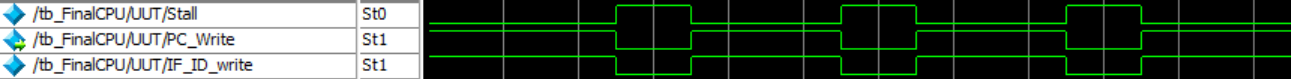
\includegraphics[width=\linewidth]{stall.png}
    \end{center}
\end{itemize}

\subsection{Forward}

\begin{itemize}
    \item \textbf{stall.asm}
    \begin{lstlisting}[language={[mips]Assembler}, frame=single]
# MEM -> EX forward
addiu   $1,     $0,     0x1111  # 0x1111
addu    $2,     $1,     $0      # 0x1111
addu    $3,     $0,     $2      # 0x1111
addu    $4,     $3,     $3      # 0x2222
# WB -> EX forward
addu    $5,     $3,     $0      # 0x1111
addu    $6,     $0,     $4      # 0x2222
addu    $7,     $5,     $5      # 0x2222
# together
addu    $7,     $7,     $7      # 0x4444
addu    $7,     $7,     $7      # 0x8888
    \end{lstlisting}

    \item \textbf{RF.out}
    \begin{lstlisting}[language={}]
00000000 // R[0]
00001111 // R[1]
00001111 // R[2]
00001111 // R[3]
00002222 // R[4]
00001111 // R[5]
00002222 // R[6]
00008888 // R[7]
...
    \end{lstlisting}

    \item 從圖中可看見各種不同forward的觸發組合:
    \begin{center}
        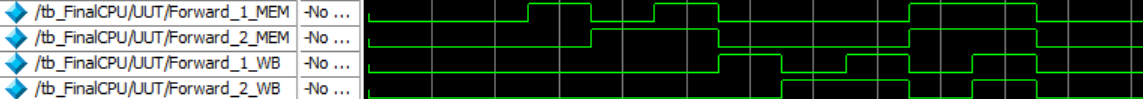
\includegraphics[width=\linewidth]{forward.png}
    \end{center}
\end{itemize}



\section{Compare with PA2}
\begin{itemize}
    \item 調整DM size = 32
    \item Area皆已去掉RF、DM、IM
    \item PA3的Slack已加上2.5
\end{itemize}
\begin{center}
\begin{tabular}{ |c|c|c|c| } 
    \hline
     & \textbf{Slack} & \textbf{Area} & \textbf{Power} \\ 
    \hline
    \textbf{PA2} & 4.3441 & 1829.548 & 2.95 mW \\ 
    \hline
    \textbf{PA3} & 4.1546 & 2938.768 & 3.24 mW \\ 
    \hline
\end{tabular}
\end{center}
理論上來說,pipeline後的最高clock cycle應該要是原本的5倍,然而事實上是Slack降低了,以下分析幾種可能的原因:
\begin{itemize}
    \item critical path的時間占比太高,導致即便將它劃分為一個pipeline區域,也不會提高整體速度。e.g. 原本的時間占比為1:1:20:1:1,總和為24個時間單位,此時即便將其拆分成五個區域,也需要配合最慢的部分,導致最後仍須要20個時間單位。
    \item 配合上一點,不僅速度沒有增加,還可能因為多出來的控制線導致延遲提高,進而降低整體slack。
    \item 或許實際電路速度確實能達到幾乎5倍的效果,但Openroad計算Slack的邏輯並非我所想的那樣,導致結果不如預期。
\end{itemize}
Area與Power的部分,因為增加了Hazard、Forward與許多Pipeline Register,導致Area與Power上升,符合預期。



\section{Memory Rethinking: Implementing Multi-level Cache}
IM與DM皆可新增Cache,以下以DM舉例:
\begin{itemize}
    \item \textbf{CPU:} 需將DM改成Cache,並判斷Cache是否miss,若是則暫停指令,直到Cache得到data之後才能繼續;若hit,則與一般的讀取/寫入動作一樣。
    \item \textbf{Cache:} 連接CPU與memory,連接CPU方面,除了需要原本DM的接腳外,還需要新增\texttt{Read\_Miss}與\texttt{Write\_Miss }2個接腳,在miss時使其變為1,得到data後才變回0;連接DM方面,則較類似CPU存取DM的行為。從外部看來類似於:
    \begin{lstlisting}[language=Verilog]
module Cache (
    // CPU方面
    input Cache_r, Cache_w,
    input [31:0] Cache_addr, Cache_w_data,
    output Read_Miss, Write_Miss,
    output [31:0] Cache_r_data,
    // DM方面
    output Mem_r, Mem_w,
    output [31:0] Mem_addr, Mem_w_data,
    intput [31:0] Mem_r_data,
);
    \end{lstlisting}
\end{itemize}

\section{Conclusion and Insights}
本次PA成功完成了pipeline CPU,老實說設計圖上的各個元件寫起來並沒有很複雜,真正痛苦的是在最後把他們接起來的時候,畢竟線實在是太多了,但這也讓我感受到腳位命名的重要性,好的命名確實能讓我快速了解一條線在圖中的位置、功能。
\par
當初在學習pipeline CPU時,還以為PA3會包含beq、j這兩個指令,這讓我十分焦慮,心想最後該不會連功能正確都無達成了吧,幸好教授與助教們大發慈悲,沒有加入這兩個指令,感恩教授、讚嘆助教!

\end{document}
